\section{Einleitung}
\label{einleitung}

\subsection{Motivation}
\label{einleitung:motivation}

Die Analyse historischer topographischer Karten ist eine bedeutende Aufgabe der Raum- und Landschaftsplanung, um die
historische Entwicklung von Siedlungen und Naturräumen nachvollziehen zu können. Besondere Aufmerksamkeit kommt dabei
der automatisierten Texterkennung zu, um digitalisiertes Kartenmaterial schnell katalogisieren, sortieren oder
durchsuchen zu können.

Die kombinierte Texterkennung in und -extraktion aus Bildern ist ein Standardproblem der Bildanalyse sowohl im Bereich
der klassischen \textit{Computer Vision} (d.h. Objekterkennung durch spezielle Algorithmen) als auch des seit einigen
Jahren populärer gewordenen Gebiet des maschinellen Lernens (siehe auch Abschnitt~\ref{einleitung:forschung}). Dieser
\gls{ocr} genannte Prozess kann in zahlreichen Anwendungsdomänen eingesetzt werden, wie etwa der automatisierten
Erkennung von Kennzeichen, der Digitalisierung von Büchern oder der Informationsextraktion aus nicht digitalisierten
Verträgen oder Business-Dokumenten.

Alle beispielhaft aufgeführten Fälle haben jedoch gemeinsam, dass die Texterkennung aufgrund des starken Kontrastes
zwischen Text und Hintergrund und des Mangels an störenden Artefakten relativ einfach möglich ist. Die Anwendung auf
historische topographische Karten gestaltet sich aufgrund einiger Faktoren vergleichsweise schwierig. So ist das
Farbspektrum trotz der Fülle an Informationen in der Regel auf die Farbe des (vergilbten) Papiers und eine einzige
Tintenfarbe eingeschränkt. Das führt dazu, dass der zu extrahierende Text sich farblich nicht von weiteren Markierungen
auf der Karte, wie etwa Straßen, Bäumen oder Höhenzügen, unterscheiden lässt und somit zahlreiche störende Objekte
bei der Erkennung ignoriert werden müssen. Darüber hinaus ist die Linienstärke der Buchstaben historischer Schriftarten
stellenweise sehr dünn, sodass dickere Linien des Bildhintergrundes weitaus dominanter erscheinen als der eigentlich
vordergründige Text (siehe Abbildung~\ref{einleitung:motivation:karten}).

Diese Schwierigkeiten machen die Texterkennung in historischen topographischen Karten zu einer besonders
herausfordernden und interessanten Aufgabe im Bereich des maschinellen Lernens.

\begin{figure}
    \centering
    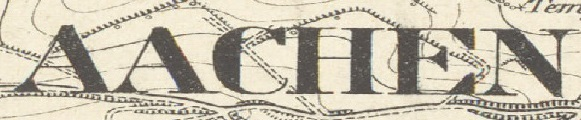
\includegraphics{img/Aachen.jpg}
    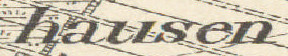
\includegraphics{img/hausen.jpg}
    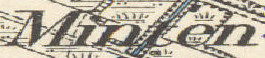
\includegraphics{img/Minten.jpg}
    \caption{Kartenbeispiele\label{einleitung:motivation:karten}}
\end{figure}

\subsection{Forschungsstand}
\label{einleitung:forschung}

Die Idee der maschinellen \gls{ocr} beschäftigt Ingenieure, Informatiker und Erfinder seit mehr als einem Jahrhundert.
Bereits 1914 stellte Edmund Fournier d'Albe ein \textit{Optophon} vor, das nach Erkennung eines Buchstabens einen
bestimmten Ton abspielte und auf diese Weise Blinden das Lesen ermöglichen sollte (vgl.~\cite{albe1914}). Wenige Jahre
später meldete der in Dresden bei der Firma \textit{Zeiss Ikon} tätige Emanuel Goldberg ein Patent für die von ihm
entwickelte \glqq statistische Maschine\grqq\ an, mit deren Hilfe die in Form von Buchstaben- und Ziffernkombinationen
vorliegenden Metadaten auf Filmrollen durchsucht werden konnten (vgl.~\cite{goldberg1931}).

In jüngerer Zeit ist die \gls{ocr} im Bereich des maschinellen Lernens häufiger untersucht worden. Eines der
bekanntesten Projekte in diesem Bereich ist die zunächst von der Firma \textit{Hewlett-Packard}, dann von der Firma
\textit{Google} entwickelte \textit{Tesseract OCR Engine} (vgl.~\cite{smith2007}), die mittlerweile neben
algorithmusbasierter Texterkennung den Einsatz eines neuronalen Netzes ermöglicht (vgl.~\cite{tesseract40}).

Jaderberg et al.\ präsentierten 2016 ein mehrstufiges Verfahren für die Texterkennung in Fotografien. Bei diesem
Verfahren wird zunächst die mögliche Existenz eines Texts in einem Bild \textit{entdeckt}. Alle Entdeckungen eines
Bildes werden der nächsten Stufe als Vorschläge präsentiert. Diese versucht dann, innerhalb der Vorschläge Text zu
\textit{erkennen}. Grundlage des Netzes ist eine Hierarchie mehrerer mit einander verbundener
\textit{convolutional layer}, an deren Ende ein \textit{fully connected layer} steht, welches die erkannten Buchstaben
ausgibt (\textit{aktiviert}) (vgl.~\cite{jaderberg2016}).

Shi et al.\ stellten 2017 ein Netzwerk vor, welches ebenfalls der Texterkennung in Fotografien dienen sollte. Wie
Jaderberg et al.\ setzen sie zunächst auf eine Hierarchie mehrerer verbundener \textit{convolutional layer}, fügen
jedoch vor der Buchstabenaktivierung \gls{lstm} \textit{layer} ein, deren Ausgabe später durch einen handgeschriebenen
Algorithmus dekodiert wird. (vgl.~\cite{shi2017})

\subsection{Zielstellung}
\label{einleitung:zielstellung}

Ziel dieser Arbeit ist der Entwurf eines neuronalen Netzes, welches Texte auf topographischen Karten erkennen und
extrahieren kann. Dieses Netz soll auf dem zur TU Dresden gehörigen HPC-System \textit{Taurus} zum Einsatz kommen und
die dort vorhandenen GPUs zur Beschleunigung verwenden.

Ferner soll das Skalierungsverhalten des Netzwerks untersucht werden, indem die Erkennungsrate des Netzes in
Abhängigkeit von der Größe der Trainingsdaten betrachtet wird.
